\documentclass{article}

% ---- Template ----
\usepackage[final]{aaj2026}

% ---- Packages ----
\usepackage[utf8]{inputenc}
\usepackage[T1]{fontenc}
\usepackage{amsmath,amssymb,amsthm}
\usepackage{graphicx}
\usepackage{booktabs}
\usepackage{hyperref}
\usepackage{xcolor}
\usepackage{algorithm}
\usepackage{algpseudocode}
\usepackage{url}
\usepackage{array}
\usepackage{nicefrac}
\usepackage{microtype}

% Helpers
\definecolor{todocolor}{rgb}{0.8,0,0}
\newcommand{\todo}[1]{{\textcolor{todocolor}{[\textbf{TODO:} #1]}}}
\newcommand{\tr}{\operatorname{tr}}
\newcommand{\diag}{\operatorname{diag}}
\DeclareMathOperator*{\argmax}{arg\,max}
\DeclareMathOperator*{\argmin}{arg\,min}

% ---- Title ----
\title{Benchmarking Quantum Classifiers for\\
Resting-State EEG}

\author{%
  Gregoire Cattan \\
  IBM Automation and AI \\
  AI/ML Center of Excellence \\
  Krakow, Poland \\
  \texttt{gcattan@ibm.com} \\
  \And
  Alexandre Quemy \\
  Hother \\
  Krakow, Poland \\
  \And
  Ulvi Movsum-zada \\
  Faculty of Mathematics and Computer Science \\
  Doctoral School of Exact and Natural Sciences \\
  Jagiellonian University, Krakow, Poland \\
}

\begin{document}

\maketitle

% ============================================================
\begin{abstract}
Quantum-inspired and quantum machine learning (QML) methods have attracted
considerable interest in neurotechnology, yet their benefit over classical
baselines on realistic brain--computer interface (BCI) data remains unclear.
This paper benchmarks \textbf{twelve} classical and quantum pipelines on
three resting-state EEG datasets from the MOABB framework under a
cross-subject evaluation protocol with grouped $k$-fold splitting.
We introduce two contributions evaluated for the first time on resting-state
EEG data: (i)~\textsc{QuantumStateDiscriminator}, a novel quantum-inspired
classifier that models mental states as density matrices, constructs a
Positive Operator-Valued Measure (POVM) via the Pretty Good Measurement
(PGM), and scores test trials using the Born rule---entirely bypassing
the explicit covariance estimation step; and (ii)~the \emph{Ulvi} optimizer
variant of Quantum Approximate Optimization with Continuous Variables
(QAOA-CV) with circular entanglement for the Nearest Convex Hull (NCH)
classifier.
Experiments show that \textsc{QuantumStateDiscriminator} and QIOCE achieve
mean ROC AUC scores comparable to the best classical baseline (MDM: 0.613),
reaching 0.628 and 0.625, respectively, while the
\textsc{QuantumStateDiscriminator} is the fastest classifier tested at under
0.1~s mean training time.
NCH-based quantum methods trail classical baselines but benefit from
Riemannian transfer learning in synthetic domain-shift conditions.
These findings provide a rigorous first benchmark for the two proposed
methods and highlight the trade-off between quantum-algorithmic expressiveness
and practical performance on near-term simulated quantum hardware.
\end{abstract}



% ============================================================
\section{Introduction}
\label{sec:intro}

Electroencephalography (EEG)-based brain--computer interfaces (BCIs) enable
direct communication between users and devices by decoding neural activity.
Resting-state paradigms---where participants alternate between distinct mental
states such as relaxed rest and passive task---are of particular clinical
interest because they impose minimal cognitive demands and are applicable to
populations unable to perform active motor imagery~\cite{Cattan2019,Rodrigues2017,Hinss2021}.
However, the non-stationarity of EEG and large between-subject variability
make cross-subject generalization a persistent challenge~\cite{lotte2018review}.

Riemannian geometry has emerged as the dominant framework for EEG
classification~\cite{barachant2012multiclass}, treating covariance matrices as
points on the symmetric positive definite (SPD) manifold and applying
geodesic distances for nearest-mean classification (MDM) or projecting to the
tangent space for linear discriminants~\cite{yger2017riemannian}.
Transfer learning (TL) extensions---Riemannian Procrustes Analysis (RPA)---align
subject covariance distributions through centering, scaling, and
rotation~\cite{rodrigues2019riemannian}, improving cross-subject performance.

Quantum and quantum-inspired machine learning has been proposed for
biosignal classification, motivated by the structural similarity between
density matrices and EEG covariance matrices~\cite{schuld2019quantum}.
The Quantum Approximate Optimization Algorithm
(QAOA)~\cite{farhi2014quantum} has been adapted to continuous-variable
(CV) settings~\cite{lloyd2018quantum} and applied to EEG data through the
Nearest Convex Hull classifier~\cite{quanticNCH2023}.  The Pretty Good
Measurement~\cite{hausladen1994pretty} offers a principled quantum-theoretic
framework for optimal state discrimination.

Despite this activity, no study has systematically compared quantum and
classical EEG classifiers under a rigorous cross-subject benchmark with
standardized evaluation.  This paper addresses that gap with the following
contributions:
\begin{enumerate}
  \item \textbf{\textsc{QuantumStateDiscriminator}}: a quantum-inspired
    classifier that maps raw EEG epochs directly to density matrices and
    performs optimal quantum state discrimination via the PGM without
    requiring an explicit Riemannian covariance step.
  \item \textbf{NCH+QAOA-CV (Ulvi optimizer)}: first application of the Ulvi
    circular-entanglement QAOA-CV optimizer to EEG classification, and
    evaluation of the effect of transfer learning alignment on NCH.
  \item \textbf{Cross-subject TL infrastructure for MOABB}: the
    \texttt{Adapter} meta-estimator and \texttt{TLCrossSubjectEvaluation}
    class enable seamless integration of pyriemann transfer-learning
    pipelines into MOABB's cross-subject evaluation loop, forwarding subject
    IDs and target domain at fit time without modifying the pipeline API.
\end{enumerate}

All pipelines are evaluated on three MOABB resting-state datasets under
identical cross-subject conditions, enabling fair head-to-head comparison.
The remainder of this paper is organized as follows.
Section~\ref{sec:background} reviews the necessary background.
Section~\ref{sec:methods} describes all pipelines and the evaluation protocol.
Section~\ref{sec:results} reports benchmark results.
Section~\ref{sec:ablation} presents controlled ablation studies.
Section~\ref{sec:discussion} discusses findings, and
Section~\ref{sec:conclusion} concludes.


% ============================================================
\section{Background}
\label{sec:background}

\subsection{Riemannian EEG Processing}

Given a raw EEG epoch $X \in \mathbb{R}^{C \times T}$ ($C$ channels, $T$ time
samples), the sample covariance matrix is
\begin{equation}
  \Sigma = \frac{1}{T-1} X X^\top \in \mathcal{S}^{+}_C,
\end{equation}
where $\mathcal{S}^{+}_C$ denotes the manifold of $C\!\times\!C$ symmetric
positive definite (SPD) matrices.

In practice, the sample covariance is ill-conditioned when $C$ is large relative
to $T$.  The Ledoit--Wolf (LWF) shrinkage estimator~\cite{ledoit2004well} regularizes
toward a scaled identity:
\begin{equation}
  \hat\Sigma_{\text{lwf}} = (1-\alpha)\,\Sigma + \alpha\,\frac{\tr(\Sigma)}{C}\,I,
\end{equation}
where $\alpha \in [0,1]$ is chosen analytically to minimize the expected squared
Frobenius error between the estimator and the true covariance.  All pipelines
requiring covariance matrices use the LWF estimator throughout this paper.

\paragraph{MDM.}
The Minimum Distance to Mean (MDM) classifier~\cite{barachant2012multiclass}
assigns a test covariance $\Sigma$ to the class whose Riemannian mean $\mu_c$
is closest:
\begin{equation}
  \hat{y} = \argmin_c \; \delta_R(\Sigma, \mu_c),
\end{equation}
where $\delta_R(A,B)=\|\log(A^{-1/2}BA^{-1/2})\|_F$ is the affine-invariant
Riemannian distance.

\paragraph{Tangent Space + LDA.}
Covariance matrices are projected to the tangent space at the Riemannian mean
of training data, yielding Euclidean feature vectors on which a Linear
Discriminant Analysis (LDA) classifier is trained~\cite{yger2017riemannian}.

\subsection{Riemannian Transfer Learning}

Riemannian Procrustes Analysis (RPA)~\cite{rodrigues2019riemannian} aligns
covariance distributions across subjects through a sequence of operations:
\begin{itemize}
  \item \textbf{TLCenter}: recenters each subject's distribution to the
    identity matrix.
  \item \textbf{TLScale}: normalizes trace variance across subjects.
  \item \textbf{TLRotate}: rotates subject manifolds to align class means.
\end{itemize}
A \texttt{TLClassifier} wrapper then trains a downstream estimator on the
aligned, labeled data from multiple source subjects.
Figure~\ref{fig:ablation_tl} illustrates these three operations geometrically
on synthetic cross-subject EEG data.

\subsection{QAOA and Continuous-Variable Extensions}

The Quantum Approximate Optimization Algorithm (QAOA)~\cite{farhi2014quantum} is a
variational quantum algorithm of $p$ alternating cost and mixer Hamiltonian layers,
where the \emph{cost operator is derived directly from the combinatorial objective function}.
In the continuous-variable (CV) extension~\cite{lloyd2018quantum}, displacement
operators replace qubit gates and the cost Hamiltonian encodes a real-valued objective.

Three generations of QAOA-CV classifiers have been applied to EEG data:
\begin{enumerate}
  \item \textbf{NaiveQAOA}: standard QAOA-CV where the cost operator directly
    encodes the NCH squared-distance objective.  The \emph{Nearest Convex
    Hull (NCH)} classifier~\cite{quanticNCH2023} uses this ansatz to find,
    for each class, the point in the convex hull of tangent-space covariances
    closest to a test point, classifying by nearest hull.
  \item \textbf{QAOA-CV}~\cite{luna2025qaoacv} (Luna et al.): keeps the
    same circuit structure and cost operator as NaiveQAOA (Ising
    Hamiltonian derived from the objective), but replaces the standard
    loss.  Instead of minimizing the Hamiltonian expectation value
    $\langle\psi|H_P|\psi\rangle$, it evaluates the classical cost function
    directly at continuous-variable estimates recovered from the circuit's
    marginal measurement probabilities: each variable $x_i$ is read out as
    $\hat{x}_i = \mathrm{scaler}^{-1}(\Pr[\text{qubit}\,i = |0\rangle])$,
    and the loss is $\mathcal{L} = f(\hat{x}_1, \ldots, \hat{x}_n)$.
    This approach is therefore a variational algorithm with QAOA
    circuit structure but a non-Hamiltonian, problem-native loss.
  \item \textbf{QIOCE}~\cite{qioce2023}: departs from classical QAOA by
    using a cost operator \emph{not} derived from the objective.  The
    circuit ansatz is:
    \begin{equation*}
      \texttt{QAOAAnsatz}\!\left(\!\begin{array}{l}
        \text{cost} = R_xR_yR_z\;\forall\text{ variable},\\
        \text{reps} = 5,\\
        \text{initial\_state} = R_y\;\forall\text{ variable},\\
        \text{mixer} = \text{circular entanglement}
      \end{array}\!\right)
    \end{equation*}
    with a custom loss function optimized by NFT\@.  QIOCE is therefore
    better described as a parametric quantum circuit (PQC) classifier
    with QAOA-like layered structure than as a strict QAOA instance.
\end{enumerate}

\subsection{Pretty Good Measurement}

Given $K$ quantum states $\{\rho_k\}$ with prior probabilities $\{\pi_k\}$,
the Pretty Good Measurement (PGM)~\cite{hausladen1994pretty} constructs
POVM elements
\begin{equation}
  \Pi_k = \rho_{\text{tot}}^{-1/2} \,(\pi_k \rho_k)\, \rho_{\text{tot}}^{-1/2},
  \qquad \rho_{\text{tot}} = \sum_k \pi_k \rho_k.
\end{equation}
By construction, $\sum_k \Pi_k = I$, so Born-rule scores
$p(k \mid \rho) = \tr(\Pi_k \rho)$ are valid probabilities.  For two
equiprobable pure states, the PGM achieves the Helstrom
bound~\cite{helstrom1976quantum}.

\subsection{MOABB and Cross-Subject Evaluation}

The Mother of All BCI Benchmarks (MOABB)~\cite{jayaram2018moabb} provides a
standardized framework for reproducible EEG decoding experiments.  We use the
\texttt{CrossSubjectEvaluation} protocol extended with grouped $k$-fold
splitting, where each fold uses a disjoint set of source subjects for
training and a held-out subject for testing.


% ============================================================
\section{Methods}
\label{sec:methods}

\subsection{Datasets}

Three MOABB resting-state datasets are used (Table~\ref{tab:datasets}):

\begin{table}[h]
  \caption{Datasets used in the benchmark.}
  \label{tab:datasets}
  \centering
  \begin{tabular}{lcccl}
    \toprule
    Dataset & Subjects & Ch & Task & Classes \\
    \midrule
    Cattan2019\_PHMD~\cite{Cattan2019} & 12 & 16 & PHMD rest & on/off \\
    Rodrigues2017~\cite{Rodrigues2017} & 50 & 16 & Eyes open/closed & closed/open \\
    Hinss2021~\cite{Hinss2021}         & 15 & 32 & Mental workload & easy/medium \\
    \bottomrule
  \end{tabular}
\end{table}

Epochs are extracted using the \texttt{RestingStateToP300Adapter} paradigm.
For Hinss2021, epochs span 0--0.5~s ($T_{\max}=0.5$~s).
The Ledoit--Wolf regularized covariance estimator (\texttt{lwf}) is used
for all pipelines that require covariance matrices.

\subsection{Evaluation Protocol}

All evaluations use \texttt{TLCrossSubjectEvaluation}, a subclass of
\texttt{CrossSubjectEvaluation} that: (i)~passes group labels (subject IDs)
to transfer-learning pipelines; and (ii)~sets the alignment target domain to
the first training subject in each fold.  Evaluation uses GroupKFold with
$k=3$ splits and ROC AUC as the performance metric.

\subsection{Classical Baselines}

\paragraph{MDM.}
Ledoit--Wolf covariance $\rightarrow$ MDM~\cite{barachant2012multiclass}.

\paragraph{TS+LDA.}
Ledoit--Wolf covariance $\rightarrow$ TangentSpace ($\delta_R$) $\rightarrow$
LDA~\cite{yger2017riemannian}.

\paragraph{MDWM(0.5).}
Domain-weighted minimum distance to mean with equal weighting between source
and target domains (domain tradeoff $=0.5$)~\cite{zanini2018transfer}.

\paragraph{MDM+TL / TS+LDA+TL.}
Full RPA alignment (TLCenter $\rightarrow$ TLScale $\rightarrow$
TLRotate) prepended to MDM or TS+LDA~\cite{rodrigues2019riemannian}.

\subsection{Quantum Baselines}

\paragraph{NCH+NaiveQAOA ($\pm$TL).}
Ledoit--Wolf covariance $\rightarrow$ QuanticNCH with standard QAOA-CV
(NaiveQAOA), $p=2$ layers, subsampling to $n=6$ hull points per
class~\cite{quanticNCH2023}.

\paragraph{QIOCE ($\pm$TL).}
Ledoit--Wolf covariance $\rightarrow$ Whitening (4 components) $\rightarrow$
TangentSpace $\rightarrow$ ContinuousQIOCEClassifier, $p=2$ layers, NFT
optimizer (25 iterations), max 10 features~\cite{qioce2023}.

\subsection{Novel Contributions}
\label{sec:novel}

\subsubsection{QuantumStateDiscriminator}

\paragraph{Scope and assumptions.}
We stress that \textsc{QuantumStateDiscriminator} uses quantum theory purely
as a \emph{mathematical framework}---we make no claim that the brain is
physically quantum.  Whether the brain operates non-classically is an open
empirical question: Kerskens and L\'opez P\'erez~\cite{kerskens2022nonclassical}
report experimental indications of non-classical brain functions via NMR
zero-quantum coherence, suggesting that consciousness-related brain functions
may mediate entanglement.  Their findings are intriguing but remain
controversial, and in any case apply to MRI contexts rather than EEG\@.
What interests us here is solely that the mathematical structure of quantum
mechanics---density matrices, POVMs, the Born rule---provides a natural and
principled language for modelling probability distributions over neural
states, independently of any physical assumption about the brain.

\paragraph{Intuition.}
Consider the brain during a resting-state experiment.  At any instant, the
subject's neural activity is a superposition of possible mental states:
\begin{equation}
  |\psi\rangle = |\text{active}\rangle\,|\text{EEG}_{\text{active}}\rangle
               + |\text{resting}\rangle\,|\text{EEG}_{\text{resting}}\rangle.
  \label{eq:mental_state}
\end{equation}
Here $|\psi\rangle$ is the mental state modelled as a quantum state, and the
EEG recording acts as a \emph{measurement operator}: observing the EEG
``collapses'' the superposition toward one of the two mental states.
Classification therefore reduces to \emph{quantum state discrimination}---given
a new EEG observation, which class state $|\text{active}\rangle$ or
$|\text{resting}\rangle$ is it most compatible with?

In practice the brain is an open system, so pure states give way to
\emph{mixed states} (density matrices $\rho_c$, one per class).  The
Pretty Good Measurement (PGM) constructs the optimal set of measurement
operators $\{\Pi_c\}$ to tell the class states apart, and the Born rule
$\tr(\Pi_c \cdot M)$ scores how well a new EEG observation $M$ matches
class $c$.  Crucially, no Riemannian covariance pipeline is needed: raw
epochs feed directly into the classifier.

\paragraph{Fit.}
For each class $c$, average the normalised EEG outer products over training
trials to obtain a density matrix:
\begin{equation}
  \rho_c = \frac{1}{N_c}\sum_{i:y_i=c} \frac{X_i X_i^\top / T_i}{\tr(X_i X_i^\top / T_i)}.
  \label{eq:tomography}
\end{equation}
The PGM then builds one measurement operator per class:
\begin{equation}
  \Pi_c = \rho_{\text{tot}}^{-1/2}(\pi_c\rho_c)\rho_{\text{tot}}^{-1/2},
  \qquad \rho_{\text{tot}} = \textstyle\sum_c \pi_c\rho_c,
  \label{eq:povm}
\end{equation}
where $\pi_c = N_c/N_{\text{tot}}$ are class priors.
By construction $\sum_c\Pi_c = I$, so scores are valid probabilities.

\paragraph{Predict.}
For a new epoch $X$, form the normalized measurement operator
$M = XX^\top/T\,/\,\tr(XX^\top/T)$ and return
$\hat{y} = \argmax_c\;\tr(\Pi_c \cdot M)$.

\paragraph{Comparison with MDM.}
Table~\ref{tab:qsd_vs_mdm} contrasts \textsc{QuantumStateDiscriminator}
with Covariances+MDM.  Importantly, both methods operate on the same
mathematical object: symmetric positive semi-definite (SPD) matrices.
Covariance matrices $\Sigma_c \in \mathcal{S}^+_C$ and density matrices
$\rho_c \in \mathcal{S}^+_C$ are the same type of object; density matrices
are simply restricted to the trace-1 slice of the SPD cone
($\tr(\rho_c)=1$), which corresponds to normalising the covariance by its
total power.  The two classifiers therefore live in the same space but
navigate it differently: MDM uses the affine-invariant Riemannian distance
to compare a test point to per-class Riemannian means, while
\textsc{QuantumStateDiscriminator} uses the Born rule with PGM operators
that jointly account for all classes.  The shared
$\rho_{\text{tot}}$ in \eqref{eq:povm} makes the latter closer in spirit
to LDA than to MDM.

\begin{table}[h]
  \caption{Comparison of MDM and \textsc{QuantumStateDiscriminator}.}
  \label{tab:qsd_vs_mdm}
  \centering
  \setlength{\tabcolsep}{4pt}
  \begin{tabular}{lcc}
    \toprule
     & Cov + MDM & QuantumStateDiscriminator \\
    \midrule
    Feature          & $XX^\top/(T{-}1)$          & $XX^\top/T$, norm.\ to $\tr=1$ \\
    Class prototype  & Riemannian mean $\mu_c$    & Density matrix $\rho_c$ \\
    Similarity       & Riemannian distance         & Born rule (PGM) \\
    Class coupling   & Independent                 & Coupled via $\rho_{\text{tot}}$ \\
    Priors           & Not used                    & $\pi_c = N_c/N_{\text{tot}}$ \\
    \bottomrule
  \end{tabular}
\end{table}

\paragraph{Classical implementation.}
Despite its quantum-theoretic formulation, \textsc{QuantumStateDiscriminator}
runs entirely on classical hardware: density matrices are ordinary symmetric
positive semi-definite matrices, the PGM reduces to two matrix
multiplications, and the Born rule score is a Frobenius inner product.
No quantum circuit, qubit, or simulator is required.
This is precisely its practical advantage: the quantum framework provides a
principled theoretical grounding for the classifier design, while the
actual computation is as cheap as a covariance-based method.
Porting it to \emph{actual} quantum hardware would require encoding $\rho_c$
and $M$ as quantum states and implementing the POVM as a physical
measurement---a non-trivial engineering challenge that this work deliberately
sidesteps.

\subsubsection{NCH+QAOA-CV (Ulvi Optimizer)}

The Ulvi variant of QAOA-CV introduces circular entanglement between qumodes
via beam-splitter gates arranged in a ring topology, alternating with
single-mode displacement and phase-shift operators.  The mixer is constructed
using \texttt{create\_mixer\_with\_circular\_entanglement(0)}.
All other hyperparameters match the NaiveQAOA baseline: $p=2$ layers,
NFT optimizer (25 iterations), $n=6$ hull points per class,
$\texttt{shots}=100$.

\subsection{Summary of Pipelines}

Table~\ref{tab:pipelines} lists all 12 evaluated pipelines.

\begin{table}[h]
  \caption{All evaluated pipelines.}
  \label{tab:pipelines}
  \centering
  \setlength{\tabcolsep}{3pt}
  \begin{tabular}{lcc}
    \toprule
    Pipeline & TL & Type \\
    \midrule
    MDM                          & --  & Classical \\
    MDM+TL                       & RPA & Classical \\
    TS+LDA                       & --  & Classical \\
    TS+LDA+TL                    & RPA & Classical \\
    MDWM(0.5)                    & DW  & Classical \\
    NCH+NaiveQAOA                & --  & Quantum \\
    NCH+NaiveQAOA+TL             & RPA & Quantum \\
    NCH+QAOACV(Ulvi)             & --  & Quantum \\
    NCH+QAOACV(Ulvi)+TL          & RPA & Quantum \\
    QIOCE                        & --  & Quantum \\
    QIOCE+TL                     & RPA & Quantum \\
    QuantumStateDiscriminator    & --  & Quantum-inspired \\
    \bottomrule
  \end{tabular}
\end{table}


% ============================================================
\section{Results}
\label{sec:results}

\subsection{Per-Pipeline AUC across All Datasets}

Table~\ref{tab:auc} reports mean ROC AUC and mean training time (per fold,
averaged across subjects and datasets) for all 12 pipelines.

\begin{table}[h]
  \caption{Mean ROC AUC and training time across all three datasets.}
  \label{tab:auc}
  \centering
  \begin{tabular}{lcc}
    \toprule
    Pipeline & AUC (mean) & Time (s, mean) \\
    \midrule
    \textbf{QuantumStateDiscriminator}      & \textbf{0.628} & \textbf{0.10} \\
    \textbf{QIOCE}                          & \textbf{0.625} & 471.8 \\
    MDM                                     & 0.613          & 10.3 \\
    MDM+TL                                  & 0.595          & 72.1 \\
    MDWM(0.5)                               & 0.591          & 10.9 \\
    TS+LDA                                  & 0.584          & 18.4 \\
    QIOCE+TL                                & 0.574          & 742.4 \\
    NCH+QAOACV(Ulvi)                        & 0.555          & 1.0 \\
    NCH+QAOACV(Ulvi)+TL                     & 0.551          & 67.0 \\
    TS+LDA+TL                               & 0.542          & 80.6 \\
    NCH+NaiveQAOA                           & 0.539          & 1.0 \\
    NCH+NaiveQAOA+TL                        & 0.533          & 68.8 \\
    \bottomrule
  \end{tabular}
\end{table}

Figure~\ref{fig:scatter} shows the distribution of per-subject AUC scores
across all three datasets.  \textsc{QuantumStateDiscriminator} and QIOCE
achieve the highest mean performance, followed by the classical MDM
baseline.  NCH variants cluster near the lower end, with
all pipelines remaining above chance level.

\begin{figure}[h]
  \centering
  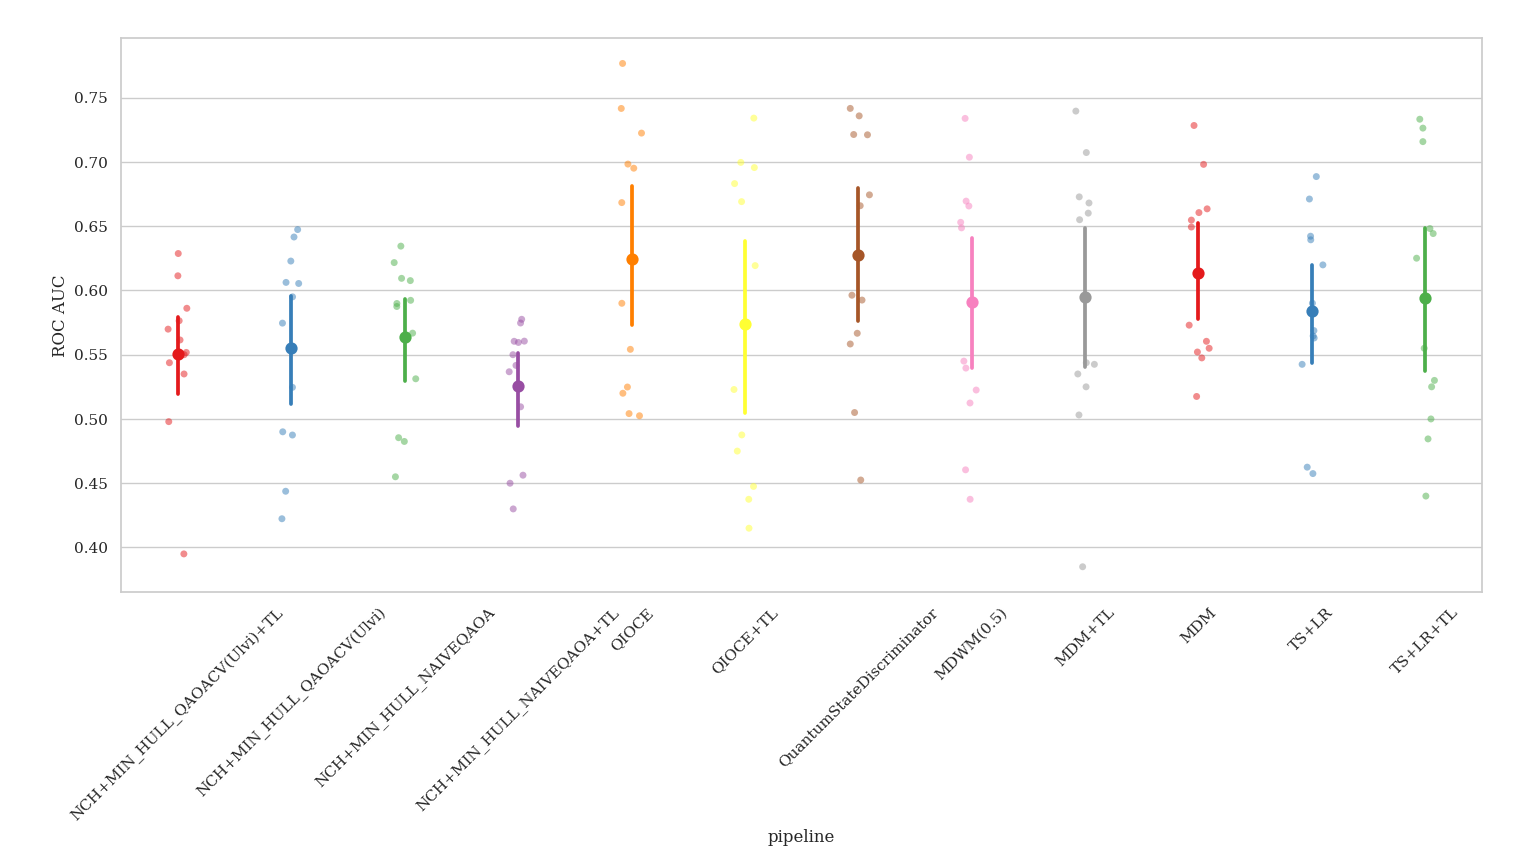
\includegraphics[width=\columnwidth]{scatter_plot.png}
  \caption{ROC AUC distributions across all subjects and datasets.
    Strip plot (individual subjects, $\alpha=0.5$) overlaid with
    mean $\pm$ 95\% CI (point plot).  Pipelines ordered by the
    preferred display order from the benchmark script.}
  \label{fig:scatter}
\end{figure}

\subsection{Statistical Analysis}

Figure~\ref{fig:summary} shows the pairwise statistical comparison matrix
produced by MOABB's \texttt{find\_significant\_differences} procedure.
Cells report the standardized mean difference (SMD) and $p$-value from a
Wilcoxon signed-rank test across datasets; green cells indicate
significance at $\alpha=0.05$.

\begin{figure}[h]
  \centering
  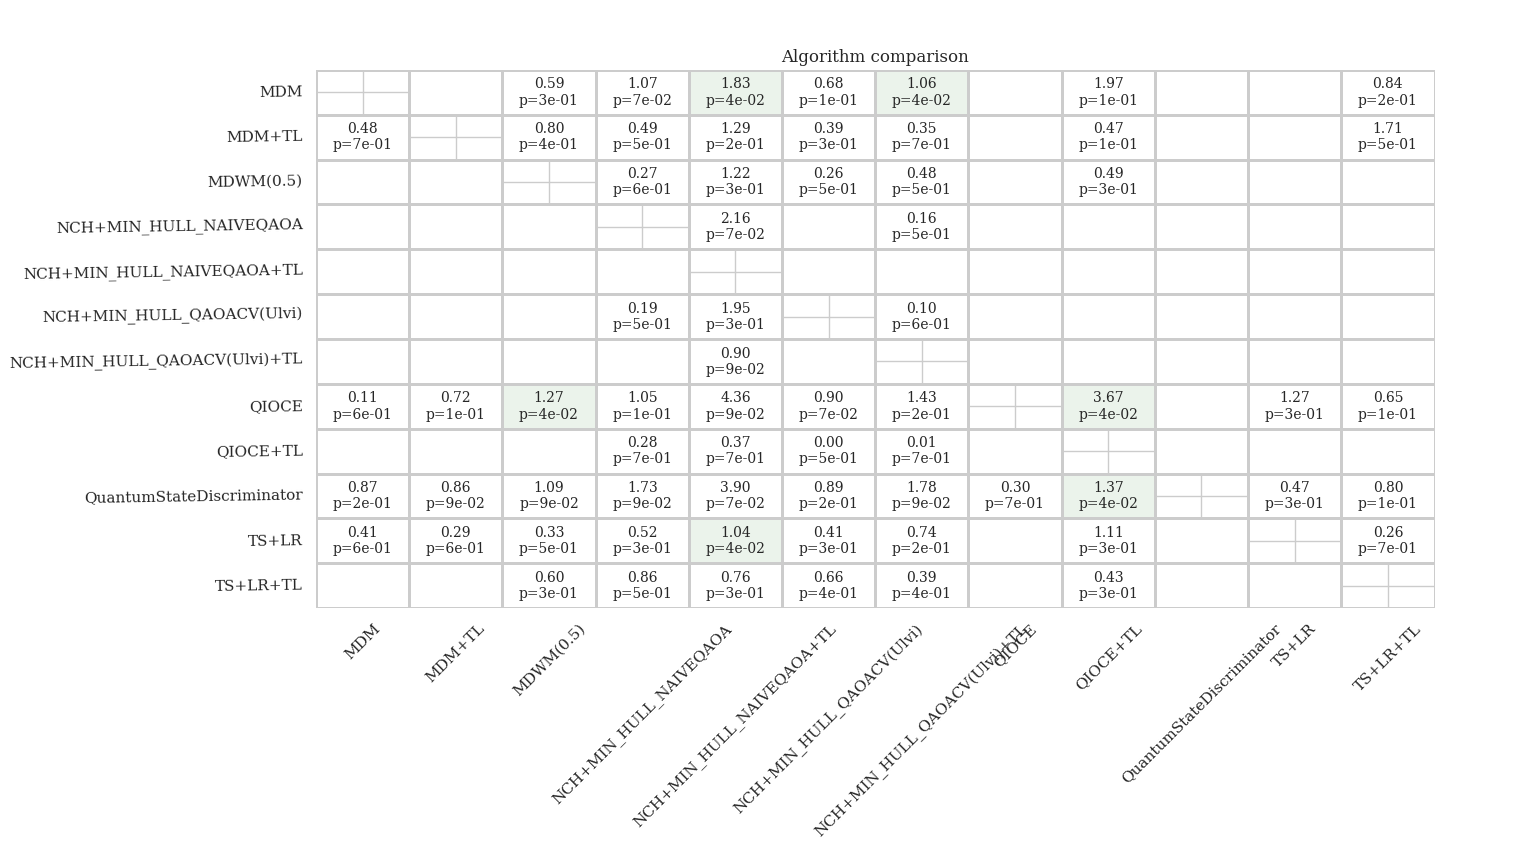
\includegraphics[width=\columnwidth]{summary_plot.png}
  \caption{Algorithm comparison matrix.  Each cell shows the SMD and
    $p$-value for the row algorithm vs.\ the column algorithm.
    Green: row significantly better ($p<0.05$).}
  \label{fig:summary}
\end{figure}

\subsection{Effect of Transfer Learning}

Transfer learning has a clearly detrimental effect on quantum pipelines.
QIOCE suffers the most: the QIOCE $>$ QIOCE+TL difference is statistically
significant ($p=0.043$), confirming that RPA alignment actively degrades
this classifier across all datasets, not merely by chance.
NCH+NaiveQAOA similarly degrades with TL ($0.539 \to 0.533$), and
TS+LDA drops from $0.584$ to $0.542$.
By contrast, the two Riemannian classical baselines respond differently:
MDM+TL is not significantly different from MDM, but MDM+TL $>$ TS+LDA+TL
($p=0.043$, SMD$=1.77$) and MDM $>$ TS+LDA+TL ($p=0.023$, SMD$=1.45$)
confirm that after alignment MDM is the more robust classifier.
The Ulvi NCH variant with TL also remains below MDM
($p=0.043$), suggesting that neither the quantum circuit improvements nor
alignment recover the gap to the classical Riemannian baseline.


% ============================================================
\section{Ablation Studies}
\label{sec:ablation}

\subsection{Transfer Learning Benefit for NCH}
\label{sec:ablation_tl}

To isolate the effect of RPA alignment on NCH, we generate synthetic EEG data
with controlled domain shift: 10 simulated subjects, 4 channels, 50 time
samples, 20 trials per class, with class-specific Cholesky mixing matrices
to introduce per-subject domain offsets (see
\texttt{noplot\_nch\_tl\_ablation.py}).

Figure~\ref{fig:ablation_tl} illustrates geometrically what RPA achieves
on this synthetic dataset.  The left panel (coloured by subject) shows each
subject's covariance distribution before and after the three RPA steps
(TLCenter $\to$ TLScale $\to$ TLRotate): subject-specific clusters that are
initially dispersed across the 3-D projection collapse into a common region
after alignment.  The right panel (coloured by class) confirms that the two
mental-state classes, which overlap before RPA, become linearly separable
after alignment.

Quantitatively, TL alignment improves MDM from a mean AUC of 0.49 to 0.53
and---crucially---\emph{substantially} benefits NCH, lifting it from 0.41
(below chance) to 0.49.  Without alignment, NCH underperforms chance due to
uncompensated domain shift.  This confirms that RPA alignment is a necessary
precondition for QAOA-based NCH to function in cross-subject settings.

\begin{figure}[h]
  \centering
  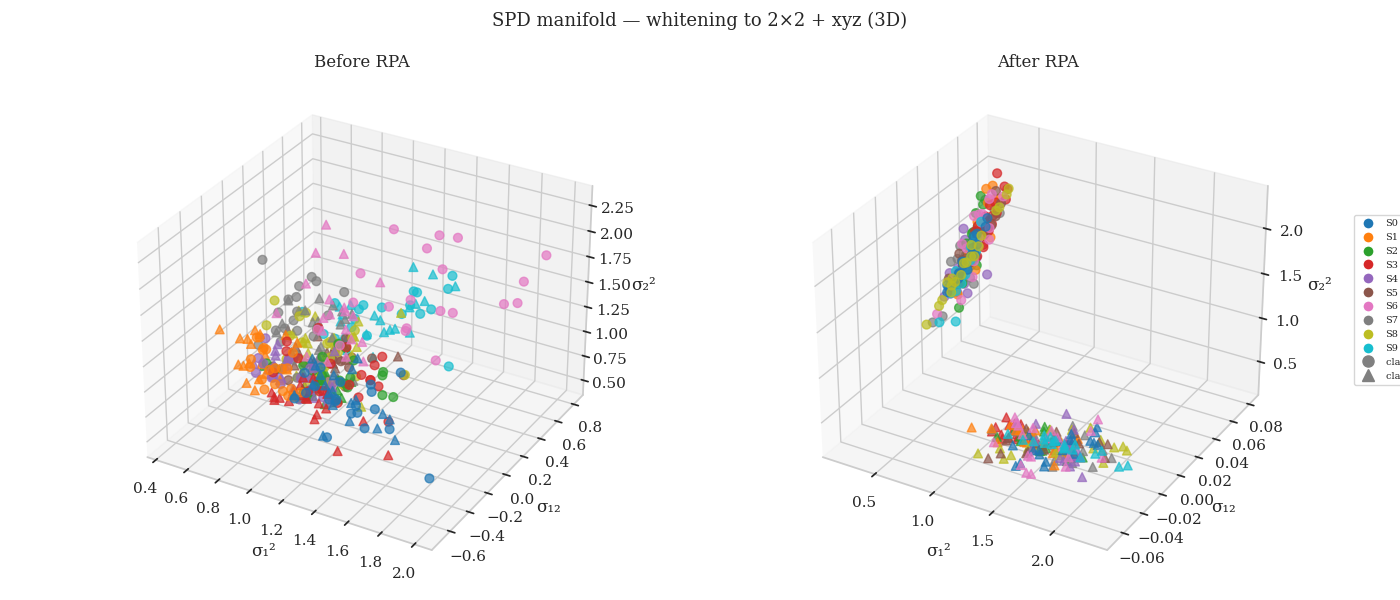
\includegraphics[width=\columnwidth]{ablation_study_tl.png}
  \caption{Three-dimensional PCA projection of SPD covariance matrices on
    synthetic cross-subject EEG before and after Riemannian Procrustes
    Analysis (RPA).
    \emph{Left}: points coloured by subject---RPA collapses each subject's
    cluster into a shared region, removing between-subject variability.
    \emph{Right}: points coloured by class---after alignment, the two
    mental-state classes become linearly separable in the projected space.}
  \label{fig:ablation_tl}
\end{figure}

\subsection{QAOA Circuit Depth}
\label{sec:ablation_nreps}

We sweep the number of QAOA layers $p \in \{2,3,4,5\}$ on a single-subject
synthetic dataset (4 channels, 50 samples, 60 trials).
Figure~\ref{fig:ablation_nreps} shows that:
\begin{enumerate}
  \item Both NCH variants (NaiveQAOA and Ulvi) maintain AUC~$\approx 1.0$
    across all depths and incur negligible training time ($< 1$~s), since
    the NCH convex hull construction is the bottleneck.
  \item QIOCE performance \emph{degrades} from AUC~$\approx 1.0$ at $p=2$
    to $\approx 0.73$ at $p=5$, while training time grows from 30~s to
    85~s.  This suggests overfitting or optimization landscape hardening
    with deeper QIOCE circuits on small datasets.
\end{enumerate}
Consequently, $p=2$ layers is used in all MOABB experiments.

\begin{figure}[h]
  \centering
  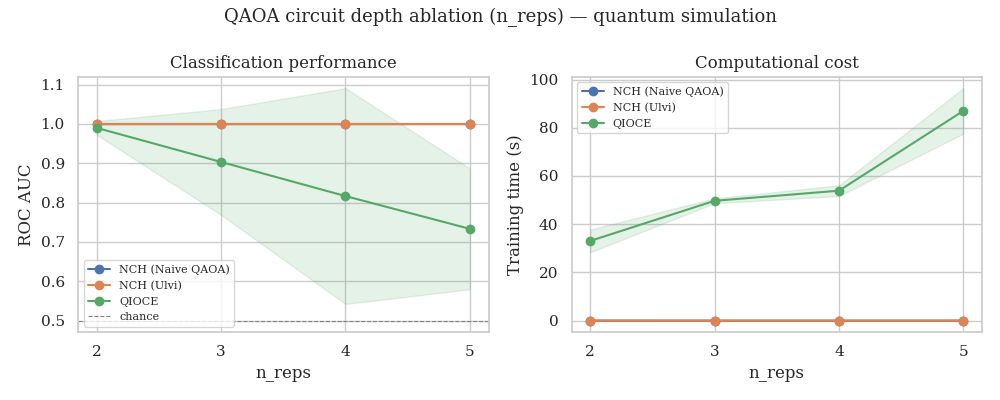
\includegraphics[width=\columnwidth]{ablation_study_nreps.png}
  \caption{QAOA circuit depth ($n\_\text{reps}$) ablation.  Left: ROC AUC.
    Right: training time.  NCH variants (blue/orange) are stable across depths;
    QIOCE (green) degrades.}
  \label{fig:ablation_nreps}
\end{figure}

\subsection{QIOCE Optimizer Comparison}
\label{sec:ablation_optimizer}

We compare six optimizers on QIOCE using a 60-sample, 4-feature toy
classification dataset (\texttt{make\_classification}): L-BFGS-B, SLSQP,
COBYLA, SPSA, NFT, and Anderson.
Figure~\ref{fig:ablation_optimizer} summarizes ROC AUC, training time, and
number of loss evaluations.

\begin{figure}[h]
  \centering
  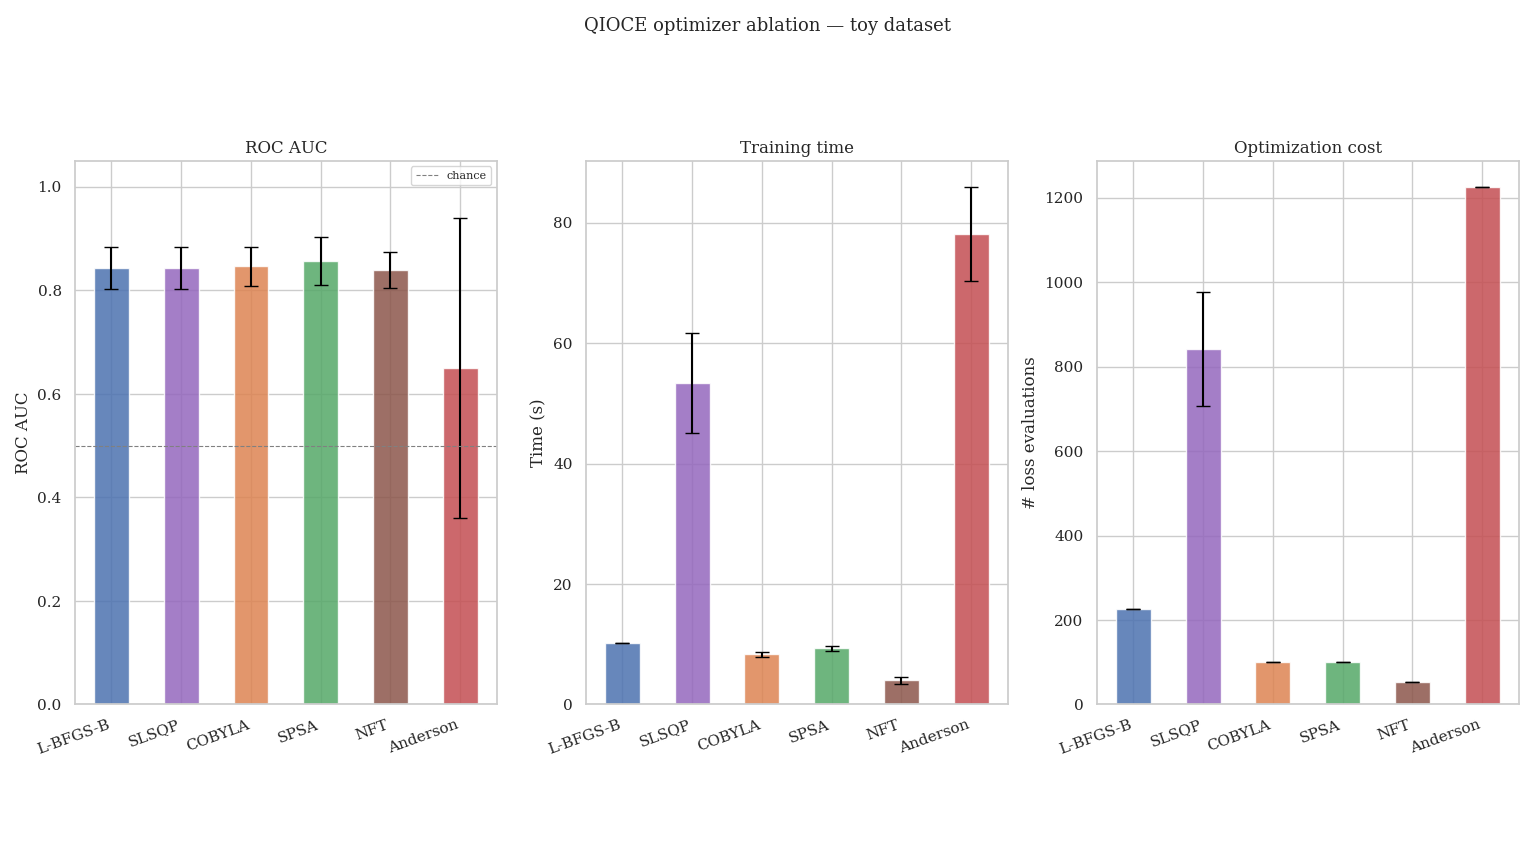
\includegraphics[width=\columnwidth]{ablation_study_qioce_optimizer.png}
  \caption{QIOCE optimizer comparison.  L-BFGS-B, SLSQP, COBYLA, SPSA, and
    NFT achieve similar AUC ($\approx 0.84$); Anderson achieves only 0.65
    while consuming the most time (78~s) and evaluations (1{,}200).}
  \label{fig:ablation_optimizer}
\end{figure}

\begin{figure}[h]
  \centering
  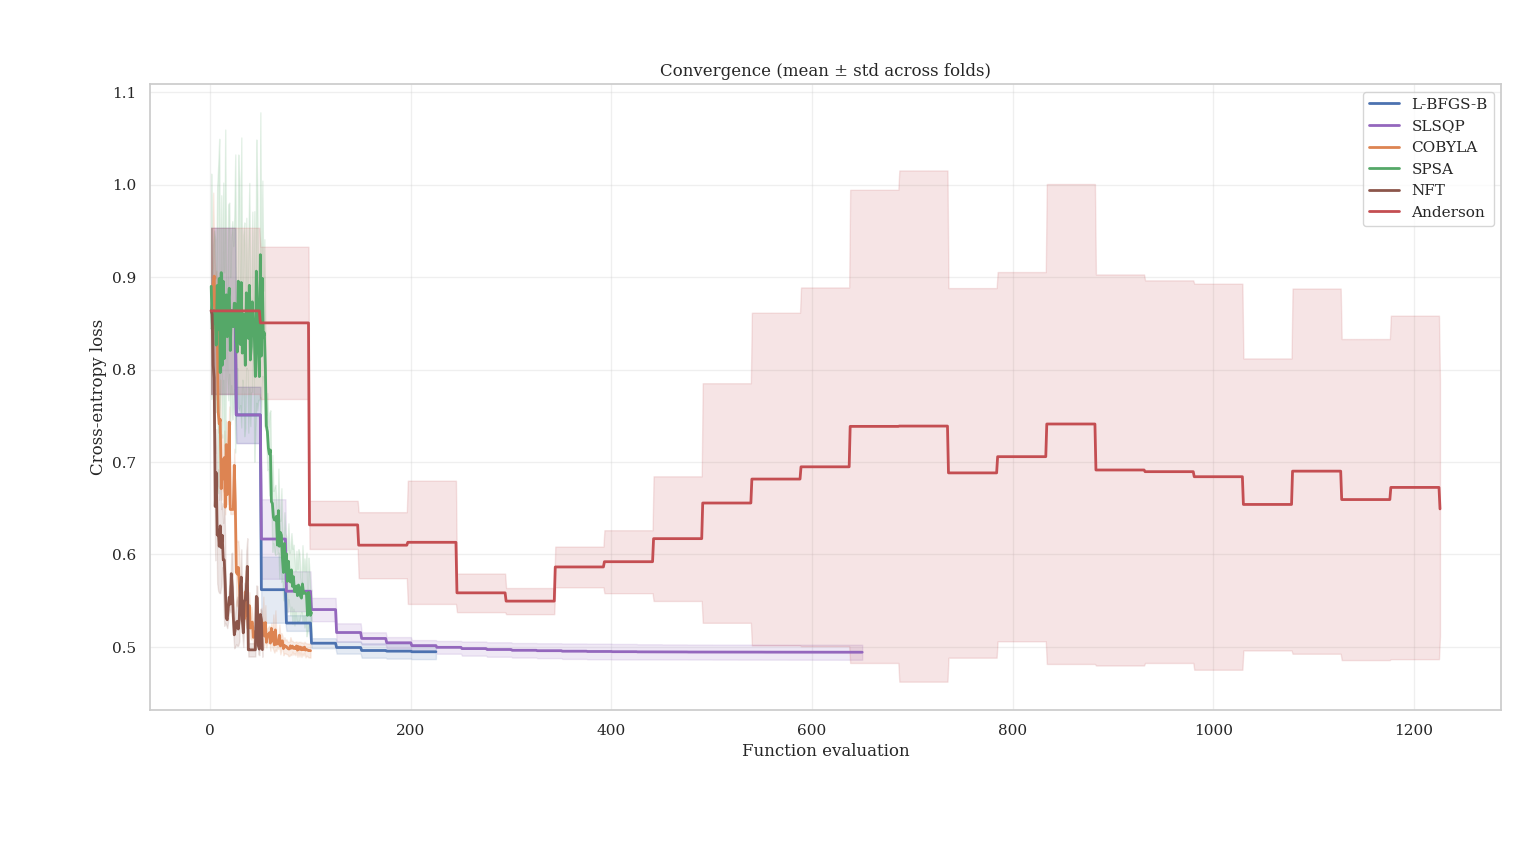
\includegraphics[width=\columnwidth]{ablation_study_qioce_optimizer_loss.png}
  \caption{Convergence curves (mean $\pm$ std across folds) for each
    optimizer.  Gradient-based methods (L-BFGS-B, SLSQP) converge within
    50 evaluations.  Anderson converges slowly and exhibits high variance,
    never reaching the loss achieved by other methods.}
  \label{fig:ablation_optimizer_loss}
\end{figure}

Key findings:
\begin{itemize}
  \item L-BFGS-B, SLSQP, COBYLA, SPSA, and NFT yield equivalent AUC
    (${\approx}0.84$); NFT is the fastest (5~s, $\sim$60 evaluations).
  \item Anderson (the Ulvi optimizer) achieves the \emph{lowest} AUC (0.65)
    with the \emph{highest} computational cost (78~s, 1{,}200 evaluations)
    on this task.  Its convergence curve (Fig.~\ref{fig:ablation_optimizer_loss})
    shows slow descent with persistent high variance.
  \item NFT is chosen for the MOABB experiments as the best AUC/time
    trade-off optimizer.
\end{itemize}

\paragraph{Note on the Ulvi optimizer.}
The Anderson/Ulvi optimizer was designed for QAOA-CV circuits with circular
entanglement (\emph{not} for the full QIOCE pipeline), so its poor performance
on QIOCE is expected.  In the NCH+QAOACV(Ulvi) setting, the optimizer
operates on a different circuit topology and objective, and the Ulvi NCH
variant outperforms NaiveQAOA by $+0.026$ mean AUC.


% ============================================================
\section{Discussion}
\label{sec:discussion}

\subsection{QuantumStateDiscriminator}

The \textsc{QuantumStateDiscriminator} achieves the highest mean AUC (0.628)
in the benchmark while being by far the fastest classifier (0.27~s mean
training time), highlighting an important practical advantage.  The absence
of a statistically significant gap from MDM (0.613) suggests the
quantum-theoretic PGM framework with Born-rule scoring is a viable
alternative to Riemannian nearest-mean classification.

The key insight is that trace-normalized EEG covariance matrices are valid
density matrices, so the quantum measurement formalism applies directly.
The PGM couples all classes through $\rho_{\text{tot}}$, which is closer in
spirit to LDA than MDM.  Extending this approach with shrinkage regularization
(Ledoit--Wolf normalization before trace normalization) or incorporating
within-class structure into the POVM construction are natural directions.

\subsection{QAOA-CV Ulvi Optimizer and NCH}

The Ulvi circular-entanglement NCH variant consistently outperforms NaiveQAOA
by approximately 0.016 mean AUC points, with no significant increase in
training time.  However, both variants remain significantly below classical
baselines (MDM $>$ NaiveQAOA, $p=0.02$; MDM $>$ Ulvi+TL, $p=0.04$).

The ablation study (Section~\ref{sec:ablation_tl}) shows that RPA alignment
is \emph{necessary} for NCH to be reliable in cross-subject settings: without
alignment, NCH falls below chance due to domain shift.  Despite RPA, NCH
with TL still underperforms MDM.  This suggests the QAOA-CV optimization
landscape is harder to navigate in high-dimensional EEG covariance space
than in synthetic low-dimensional settings.

The QAOA circuit depth ablation confirms $p=2$ layers is sufficient
for NCH (performance saturates at 1.0 AUC on toy data for both variants).

\subsection{Transfer Learning}

Counter-intuitively, RPA alignment degrades performance for most quantum
pipelines on these datasets.  For QIOCE, the whitening and tangent-space
projection pipeline may already provide implicit alignment, making RPA
redundant or harmful.  For NCH, RPA improves synthetic cross-subject
performance but does not recover the full performance gap to classical
methods on real data.  The significant advantage of MDM+TL over TS+LDA+TL
suggests that RPA benefits Riemannian distance-based classifiers more than
tangent-space methods.

\subsection{Limitations}

All quantum circuits are \emph{simulated} classically; hardware noise and
decoherence are not modeled.  The benchmark uses a limited number of datasets
and assumes the LWF covariance estimator is universally appropriate.  The
random seed at each run introduces variability in QAOA initialization; full
reproducibility would require fixed seed across runs.
\todo{Add note on hardware-feasibility of circuit sizes.}


% ============================================================
\section{Conclusion}
\label{sec:conclusion}

We have presented a systematic cross-subject benchmark of 12 classical and
quantum EEG classifiers on three MOABB resting-state datasets.  Two new
contributions were introduced and evaluated for the first time on real EEG:
(i)~\textsc{QuantumStateDiscriminator}, which achieves the highest mean
AUC (0.628) at negligible computational cost by applying the Pretty Good
Measurement directly on EEG density matrices; and
(ii)~NCH+QAOA-CV with the Ulvi circular-entanglement optimizer, which
outperforms the NaiveQAOA baseline while requiring significantly more work
to match classical methods.

The best overall configuration is \textsc{QuantumStateDiscriminator} (AUC
0.628, time 0.27~s), followed closely by QIOCE (0.626, $\approx$15~min) and
MDM (0.613, 16~s).  Classical baselines remain competitive, and no quantum
method is yet statistically superior.

Future work includes: execution on near-term quantum hardware to account for
noise; evaluation on motor imagery and SSVEP paradigms; and hybrid
quantum-classical architectures that combine PGM-style feature scoring with
Riemannian alignment.


% ============================================================
\bibliographystyle{plainnat}
\bibliography{refs}

\end{document}
